\documentclass[tikz,border=2pt]{standalone}
\usepackage{pgfplots}
\usetikzlibrary{intersections}
\usepgfplotslibrary{fillbetween}
\pgfplotsset{compat=1.7}

\begin{document}
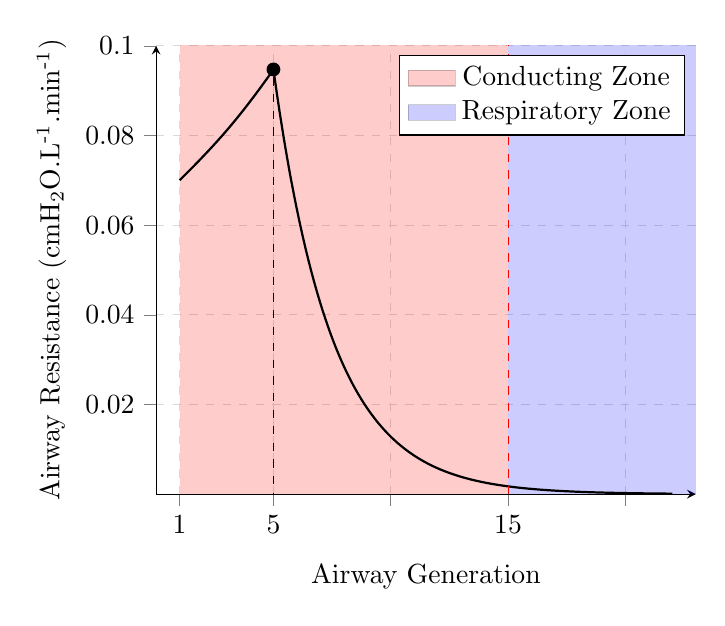
\begin{tikzpicture}
    \begin{axis}[
        axis x line=middle,
        axis y line=middle,
        grid = major,
        grid style={dashed, gray!30},
    	  x label style={at={(axis description cs:0.5,-0.1)},anchor=north},
	  y label style={at={(axis description cs:-0.1,.5)},rotate=90,anchor=south,precision=2},
	  xticklabels={},
	  yticklabels={,,0.02,0.04,0.06,0.08,0.1},
	extra x ticks={1, 5,15},
        xmin=0,
        xmax= 23,
        ymin= 0,
        ymax= 1,
	 ylabel near ticks,
	xlabel near ticks,
        xlabel=Airway Generation,
        ylabel=Airway Resistance (cmH\textsubscript{2}O.L\textsuperscript{-1}.min\textsuperscript{-1}),
        tick align=outside,
        enlargelimits=false]

	\coordinate (o) (0,0);
	\addplot[domain=5:22, black, thick,samples=500,forget plot] {7*e^(-0.4*x)} node[name=node1, circle,fill=black,inner sep=0pt,minimum size=5pt,pos=0]{};
	\draw [black, thin, dashed,] (node1) -- (node1 |- o);
	\path [black, thick, bend right=5] (10, 70) edge (50, 94.7);

\draw[name path=left, opacity=0] (axis cs: 1,0) -- (axis cs: 1,100);
\draw[name path=middle, red, thin, dashed] (axis cs: 15,0) -- (axis cs: 15,100);
\addplot[fill=red,opacity=0.2] fill between [of=left and middle];
\draw[name path=right, opacity=0] (axis cs: 23,0) -- (axis cs: 23,100);
\addplot[fill=blue,opacity=0.2] fill between [of=middle and right];
\addlegendentry{Conducting Zone};
\addlegendentry{Respiratory Zone};



\end{axis}

\end{tikzpicture} 
\end{document}